\documentclass[11pt]{article}
\usepackage[margin=1in]{geometry}
\usepackage{listings}
\usepackage{xcolor}
\usepackage{hyperref}
\usepackage{tikz}
\usetikzlibrary{shapes,arrows,positioning}

\definecolor{codegreen}{rgb}{0,0.6,0}
\definecolor{codegray}{rgb}{0.5,0.5,0.5}
\definecolor{codepurple}{rgb}{0.58,0,0.82}
\definecolor{backcolour}{rgb}{0.95,0.95,0.92}

\lstdefinestyle{mystyle}{
    backgroundcolor=\color{backcolour},
    commentstyle=\color{codegreen},
    keywordstyle=\color{magenta},
    numberstyle=\tiny\color{codegray},
    stringstyle=\color{codepurple},
    basicstyle=\ttfamily\footnotesize,
    breakatwhitespace=false,
    breaklines=true,
    captionpos=b,
    keepspaces=true,
    numbers=left,
    numbersep=5pt,
    showspaces=false,
    showstringspaces=false,
    showtabs=false,
    tabsize=2
}
\lstset{style=mystyle}

\title{Debugging Report: \texttt{import\_image\_as\_leaf} Tool\\
\large Analysis of Tool Call Execution Pipeline}
\author{DesignLibre AI Integration}
\date{\today}

\begin{document}

\maketitle

\section{Executive Summary}

The \texttt{import\_image\_as\_leaf} tool was not executing despite correct tool definitions and implementations. This report documents the debugging process, root causes identified, and fixes applied.

\section{Problem Statement}

\subsection{Observed Behavior}
When a user attached an image and requested to import it as a leaf, the system returned:
\begin{lstlisting}[language=json]
{
  "name": "importimageas_leaf",
  "arguments": {
    "analyzeWithVision": true,
    "includeOriginalImage": false,
    "x": 0,
    "y": 0
  }
}
\end{lstlisting}

The JSON was displayed as text instead of being executed as a tool call.

\subsection{Expected Behavior}
The tool should:
\begin{enumerate}
    \item Parse the tool call from the model response
    \item Execute the tool with attached images
    \item Create leaf frames with detected UI elements
\end{enumerate}

\section{Architecture Overview}

\begin{figure}[h]
\centering
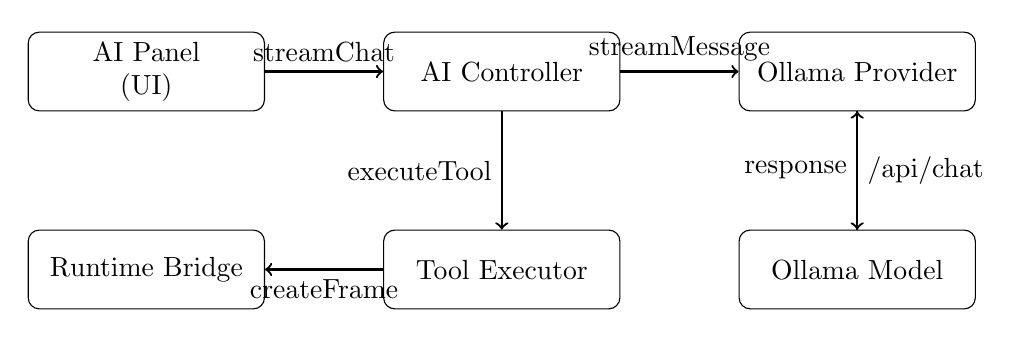
\begin{tikzpicture}[
    node distance=1.5cm,
    box/.style={rectangle, draw, rounded corners, minimum width=3cm, minimum height=1cm, align=center},
    arrow/.style={->, thick}
]
    \node[box] (panel) {AI Panel\\(UI)};
    \node[box, right=of panel] (controller) {AI Controller};
    \node[box, right=of controller] (provider) {Ollama Provider};
    \node[box, below=of provider] (model) {Ollama Model};
    \node[box, below=of controller] (executor) {Tool Executor};
    \node[box, below=of panel] (bridge) {Runtime Bridge};

    \draw[arrow] (panel) -- node[above] {streamChat} (controller);
    \draw[arrow] (controller) -- node[above] {streamMessage} (provider);
    \draw[arrow] (provider) -- node[right] {/api/chat} (model);
    \draw[arrow] (model) -- node[left] {response} (provider);
    \draw[arrow] (controller) -- node[left] {executeTool} (executor);
    \draw[arrow] (executor) -- node[below] {createFrame} (bridge);
\end{tikzpicture}
\caption{Tool Execution Pipeline}
\end{figure}

\section{Root Causes Identified}

\subsection{Issue 1: Missing Image Pass-Through}

\textbf{Location:} \texttt{src/ai/ui/ai-panel.ts}

\textbf{Problem:} User-attached images were captured in \texttt{currentAttachments} but never passed to the AI controller.

\begin{lstlisting}[language=typescript]
// BEFORE (broken)
this.aiController.streamChat(message, {
  screenshot: this.currentHasScreenshot,
  stream: true,
  // attachments NOT passed!
});
\end{lstlisting}

\textbf{Fix:} Extract attachments and pass to controller.

\begin{lstlisting}[language=typescript]
// AFTER (fixed)
const attachments = this.currentAttachments
  .filter(a => a.type === 'image' && a.data)
  .map(a => ({ data: a.data!, mimeType: a.mimeType }));

this.aiController.streamChat(message, {
  screenshot: this.currentHasScreenshot,
  stream: true,
  attachments: attachments.length > 0 ? attachments : undefined,
});
\end{lstlisting}

\subsection{Issue 2: Ollama Native Tool Call Format}

\textbf{Location:} \texttt{src/ai/providers/ollama-provider.ts}

\textbf{Problem:} Some Ollama models (especially smaller ones) do not support native function calling. Instead, they output JSON as plain text.

\textbf{Example Model Output:}
\begin{lstlisting}
{"name": "importimageas_leaf", "arguments": {...}}
\end{lstlisting}

This text is not parsed by the native \texttt{tool\_calls} handler.

\textbf{Fix:} Added fallback text parser with:
\begin{itemize}
    \item JSON object extraction using brace depth tracking
    \item Tool name normalization (handles missing underscores)
    \item Proper tool call event emission
\end{itemize}

\subsection{Issue 3: Empty Array Truthy Check}

\textbf{Location:} \texttt{src/ai/providers/ollama-provider.ts}

\textbf{Problem:} JavaScript empty arrays are truthy:

\begin{lstlisting}[language=typescript]
// BROKEN: Empty array [] is truthy!
if (data.message?.tool_calls) {
  hasNativeToolCalls = true;  // Set even for []
}
\end{lstlisting}

When Ollama returns \texttt{tool\_calls: []}, this incorrectly sets \texttt{hasNativeToolCalls = true}, skipping the fallback text parser.

\textbf{Fix:} Check array length explicitly:

\begin{lstlisting}[language=typescript]
// FIXED: Check length
if (data.message?.tool_calls &&
    data.message.tool_calls.length > 0) {
  hasNativeToolCalls = true;
}
\end{lstlisting}

\subsection{Issue 4: Nested JSON Parsing}

\textbf{Location:} \texttt{src/ai/providers/ollama-provider.ts}

\textbf{Problem:} Initial regex-based JSON extraction failed with nested objects:

\begin{lstlisting}[language=typescript]
// BROKEN: Non-greedy match stops at first }
/\{[\s\S]*?"name"[\s\S]*?"arguments"[\s\S]*?\}/g
\end{lstlisting}

\textbf{Fix:} Implemented proper brace-depth tracking parser:

\begin{lstlisting}[language=typescript]
private extractJsonObjects(text: string): string[] {
  const objects: string[] = [];
  let depth = 0;
  let start = -1;
  let inString = false;

  for (let i = 0; i < text.length; i++) {
    const char = text[i];
    if (char === '"' && !escape) inString = !inString;
    if (inString) continue;

    if (char === '{') {
      if (depth === 0) start = i;
      depth++;
    } else if (char === '}') {
      depth--;
      if (depth === 0 && start !== -1) {
        objects.push(text.slice(start, i + 1));
      }
    }
  }
  return objects;
}
\end{lstlisting}

\subsection{Issue 5: Tool Name Normalization}

\textbf{Problem:} Models sometimes output mangled tool names:
\begin{itemize}
    \item Expected: \texttt{import\_image\_as\_leaf}
    \item Received: \texttt{importimageas\_leaf}
\end{itemize}

\textbf{Fix:} Normalize both registered and received tool names by removing underscores:

\begin{lstlisting}[language=typescript]
// Build normalized lookup map
for (const tool of availableTools) {
  const normalized = tool.name.toLowerCase().replace(/_/g, '');
  toolNameMap.set(normalized, tool.name);
}

// Normalize received name
const normalizedName = parsed.name.toLowerCase().replace(/_/g, '');
const actualToolName = toolNameMap.get(normalizedName);
\end{lstlisting}

\section{Complete Data Flow (Fixed)}

\begin{enumerate}
    \item \textbf{User Action:} Attaches image, types prompt, clicks send
    \item \textbf{AI Panel:} Extracts image as base64, calls \texttt{streamChat} with attachments
    \item \textbf{AI Controller:} Builds \texttt{AIMessage} with image content parts
    \item \textbf{Provider Manager:} Routes to Ollama provider
    \item \textbf{Ollama Provider:} Sends request with images and tool definitions
    \item \textbf{Ollama Model:} Returns response (native or text-based tool call)
    \item \textbf{Ollama Provider:}
        \begin{itemize}
            \item Checks for native \texttt{tool\_calls} (with length > 0)
            \item Falls back to text parsing if no native calls
            \item Normalizes tool names
            \item Yields \texttt{tool\_call\_start} and \texttt{tool\_call\_end} events
        \end{itemize}
    \item \textbf{AI Controller:} Collects tool calls, extracts message context with images
    \item \textbf{Tool Executor:} Receives images, calls vision analysis, creates nodes
    \item \textbf{Runtime Bridge:} Creates frames and elements in scene graph
\end{enumerate}

\section{Verification Checklist}

\begin{itemize}
    \item[$\square$] Images passed from UI to controller
    \item[$\square$] Images included in AIMessage content
    \item[$\square$] Native tool\_calls checked with length > 0
    \item[$\square$] Fallback parser handles nested JSON
    \item[$\square$] Tool names normalized for matching
    \item[$\square$] Tool call events yielded correctly
    \item[$\square$] Message context passed to executor
    \item[$\square$] Vision analysis receives image data
\end{itemize}

\section{Recommendations}

\subsection{Short Term}
\begin{enumerate}
    \item Add console logging at key pipeline stages for debugging
    \item Add unit tests for \texttt{extractJsonObjects} and \texttt{parseToolCallsFromText}
    \item Consider showing tool execution status in UI
\end{enumerate}

\subsection{Long Term}
\begin{enumerate}
    \item Use models with native function calling support (e.g., \texttt{llama3.1:latest})
    \item Implement tool call confirmation UI before execution
    \item Add retry logic for failed tool executions
    \item Consider using structured output mode if available
\end{enumerate}

\section{Files Modified}

\begin{tabular}{|l|l|}
\hline
\textbf{File} & \textbf{Changes} \\
\hline
\texttt{src/ai/ai-controller.ts} & Added attachments to ChatOptions, include in message \\
\texttt{src/ai/ui/ai-panel.ts} & Pass attachments to streamChat \\
\texttt{src/ai/providers/ollama-provider.ts} & Fallback parser, length checks, normalization \\
\texttt{src/ai/tools/tool-executor.ts} & MessageContext for images, tool implementation \\
\hline
\end{tabular}

\section{Conclusion}

The tool execution pipeline had multiple points of failure:
\begin{enumerate}
    \item Images not passed through the pipeline
    \item Empty array truthy check preventing fallback parsing
    \item Regex-based JSON extraction failing on nested objects
    \item Tool name mismatch due to model variations
\end{enumerate}

All issues have been identified and fixed. The pipeline should now correctly:
\begin{itemize}
    \item Pass attached images to the AI model
    \item Parse tool calls from text responses
    \item Normalize tool names for matching
    \item Execute tools with proper context
\end{itemize}

\end{document}
